\chapter{Proces predaja}

Keďže neplánujem vytvárať klasický e-shop, namiesto procesa predaja produktu som vytvoril ECC (obrázky \ref{ecc:1}, \ref{ecc:2}, \ref{ecc:3}) diagram a RACI maticu pomocou tabuľky \ref{raci}, ktoré znázorňujú proces predaja služby nasadenia informačného systému s pomocou Kubernetes a ďalšie doplňujúce služby.


\begin{figure}[htbp]
  \centering
  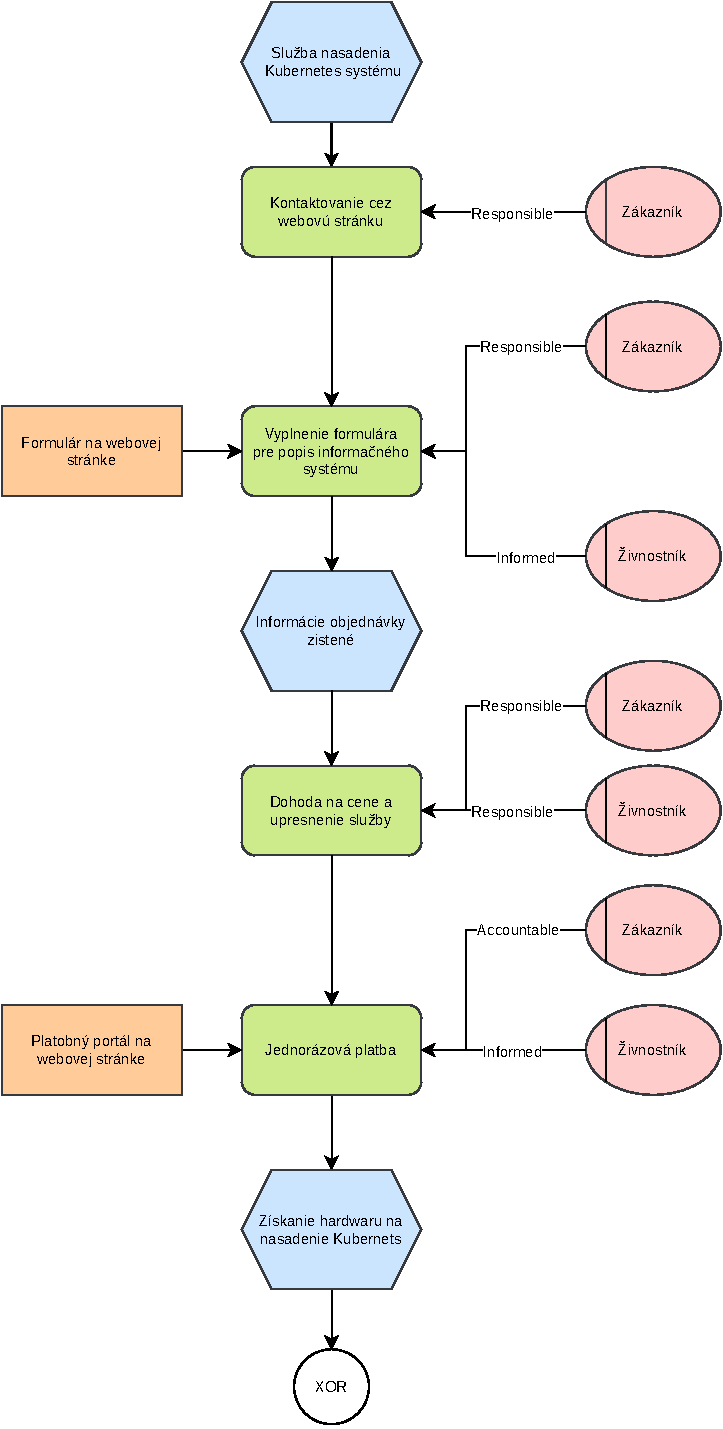
\includegraphics[width=0.5\textwidth]{images/EPC_1.pdf}
  \caption{EPC Prvá časť}
  \label{ecc:1}
\end{figure}

\begin{figure}[htbp]
  \centering
  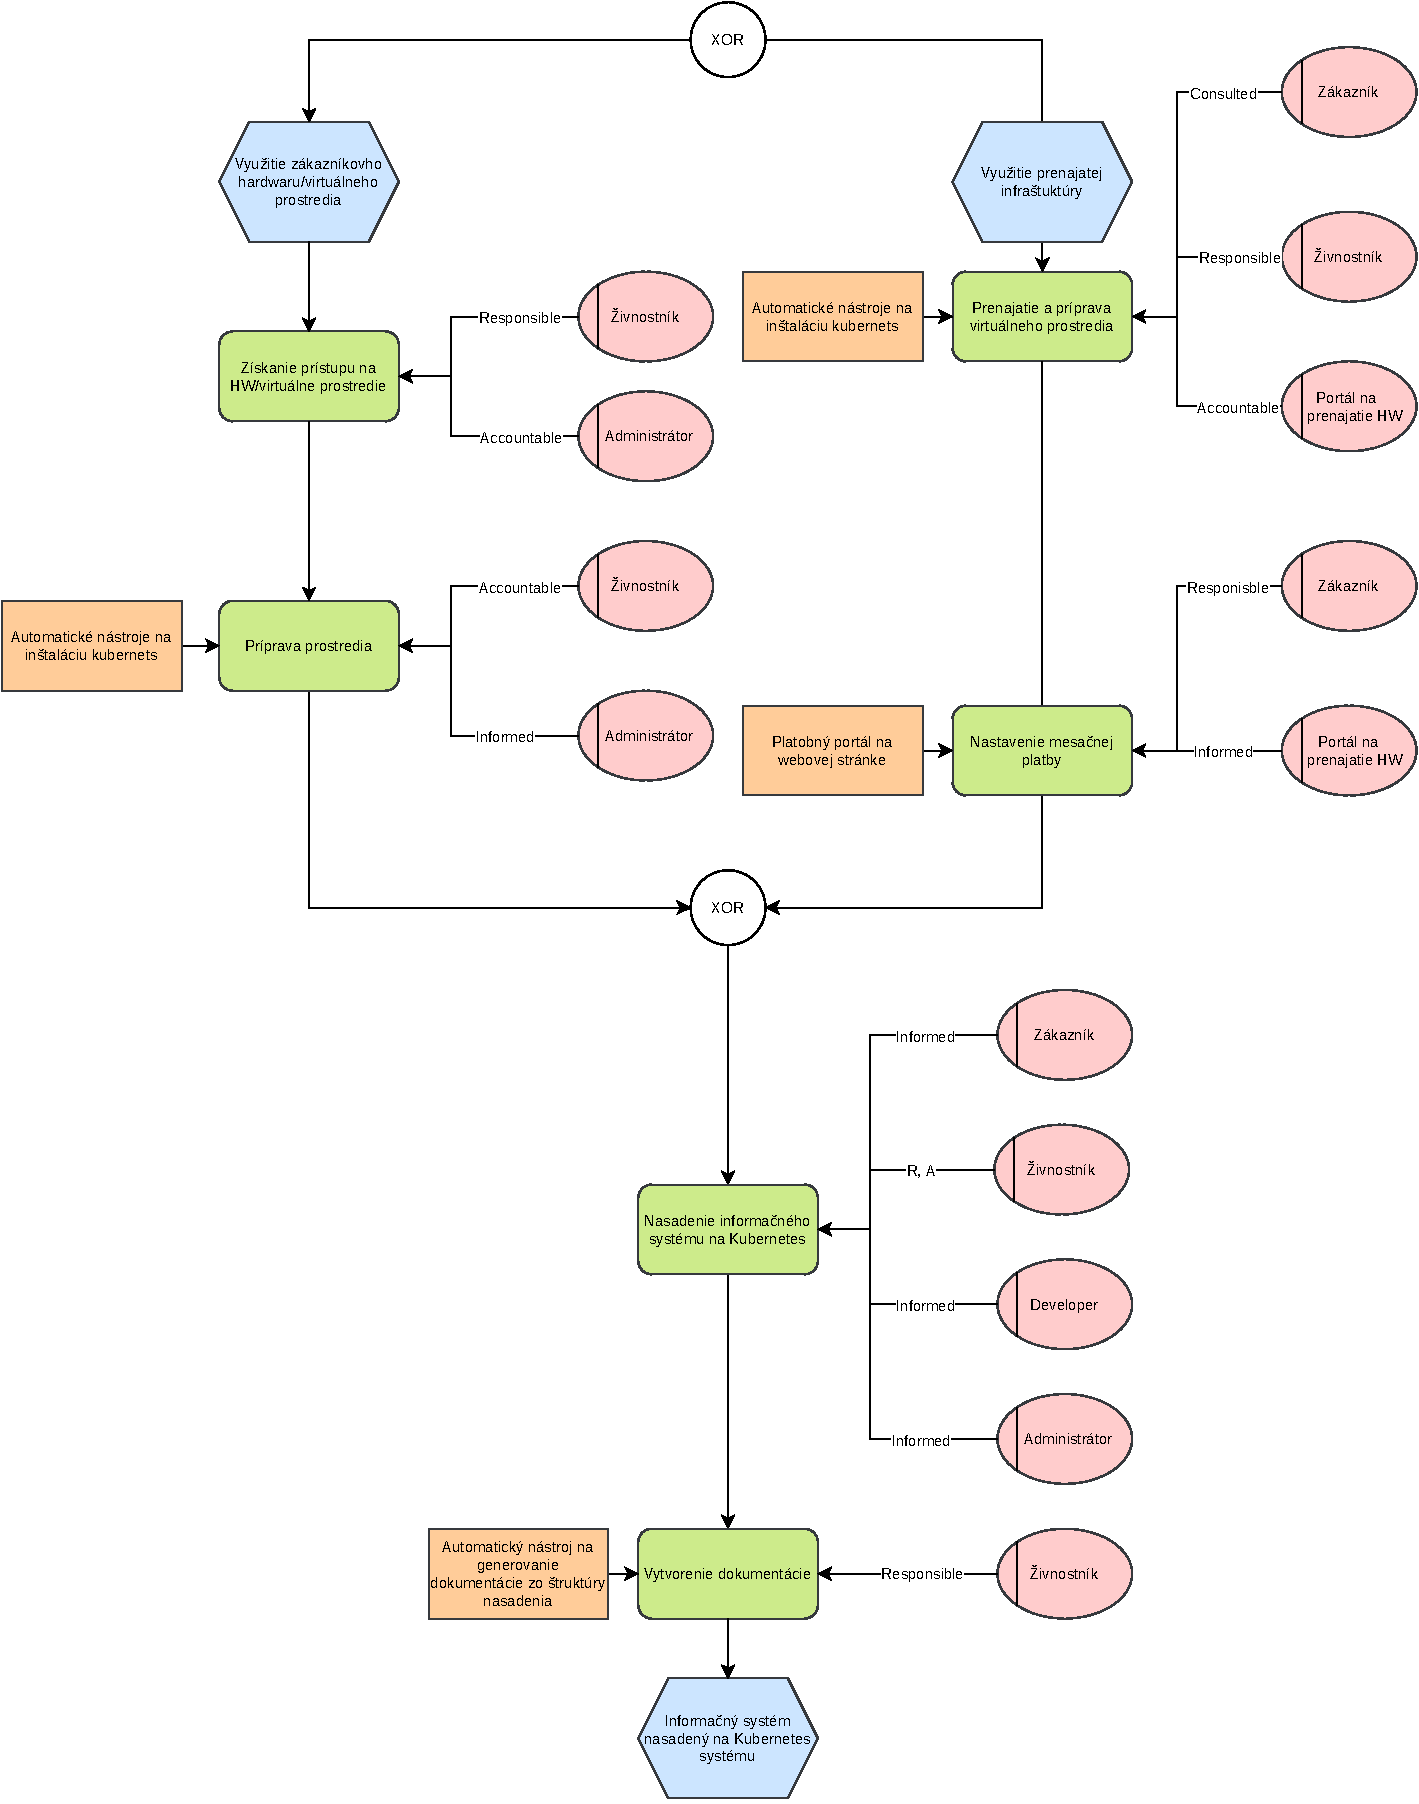
\includegraphics[width=\textwidth]{images/EPC_2.pdf}
  \caption{EPC Druhá časť}
  \label{ecc:2}
\end{figure}

\begin{figure}[htbp]
  \centering
  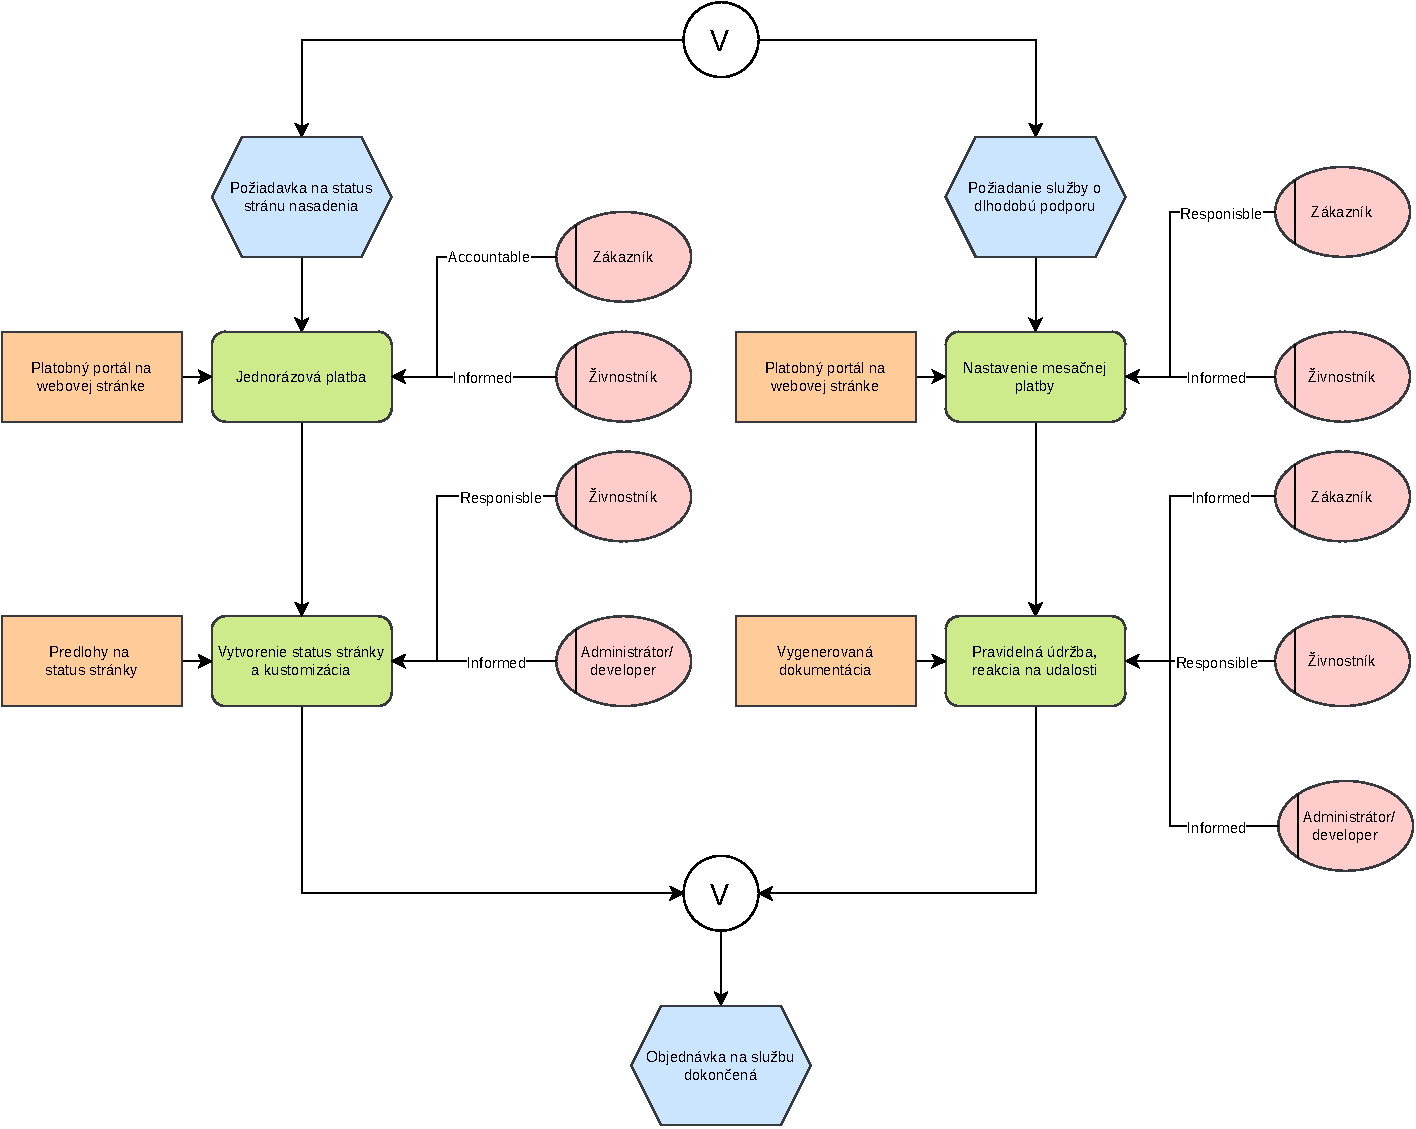
\includegraphics[width=\textwidth]{images/EPC_3.pdf}
  \caption{EPC Tretia časť}
  \label{ecc:3}
\end{figure}

\begin{landscape}
\begin{table}[htbp]
  \centering
  \begin{tabular}{|l|c|c|c|c|c|c|}
      \hline
      & \multirow{2}*{\textbf{Procesné role}} & \multirow{4}*{\textbf{Živnostník}} & \multirow{4}*{\textbf{Zákazník}} & \multirow{4}*{\textbf{Administrátor}} & \multirow{4}*{\textbf{Developer}} & \multirow{4}*{\textbf{HW portál}}\\
       &  &  &  &  &  & \\
       \cline{1-2}\multirow{2}*{\textbf{Popis aktivity}} &  &  &  &  &  & \\
       &  &  &  &  &  & \\
      \hline 
      \multicolumn{2}{|l|}{Kontaktovanie cez webovú stránku} &  & R &  &  & \\
      \hline 
      \multicolumn{2}{|l|}{Vyplnenie formulára pre popis informačného systému} & I & R &  &  & \\
      \hline 
      \multicolumn{2}{|l|}{Dohoda na cene a upresnenie služby} & R & R &  &  & \\
      \hline 
      \multicolumn{2}{|l|}{Jednorázová platba} & I & A &  &  & \\
      \hline 
      \multicolumn{2}{|l|}{Získanie prístupu na HW/virtuálne prostredie} & R &  & A &  & \\
      \hline 
      \multicolumn{2}{|l|}{Príprava prostredia} & A &  & I &  & \\
      \hline 
      \multicolumn{2}{|l|}{Prenajatie a príprava virtuálneho prostredia} & R & C &  &  & A\\
      \hline 
      \multicolumn{2}{|l|}{Nastavenie mesačnej platby} &  & R &  &  & I\\
      \hline 
      \multicolumn{2}{|l|}{Nasadenie informačného systému na Kubernetes} & R, A & I & I & I & \\
      \hline 
      \multicolumn{2}{|l|}{Vytvorenie dokumentácie} & R &  &  &  & \\
      \hline 
      \multicolumn{2}{|l|}{Vytvorenie status stránky a kustomizácia} & R &  & I &  & \\
      \hline 
      \multicolumn{2}{|l|}{Pravidelná údržba, reakcia na udalosti} & R & I & I &  & \\
      \hline 
  \end{tabular}
  \caption{RACI matica}
  \label{raci}
\end{table}
\end{landscape}
